\chapter{Background \& Related Work}


\section{Generative Adversarial Networks} \label{GAN}
Generative Adversarial Network(GANs)\cite{goodfellow2014generative} has become a global phenomenon in deep learning algorithms. The algorithm uses two networks, Generators and Discriminators, in a minimax algorithm situation where both of them tries to outperform another in a significant task e.g. image generation \cite{DBLP:journals/corr/RadfordMC15} \cite{DBLP:journals/corr/DentonCSF15}, image editing\cite{DBLP:journals/corr/ZhuKSE16}, text2image\cite{DBLP:journals/corr/ZhangXLZHWM16}, image inpainting\cite{DBLP:journals/corr/PathakKDDE16}, image-to-image translation tasks\cite{cyclegan} \cite{pix2pix} etc. Full objective of GAN function is:
\begin{align}
\min_G \max_D V(D, G)=\mathbb{E}_{x\sim p_{data}(x)}[\log D(x)] + \mathbb{E}_{z\sim p_z(z)}[\log(1 - D(G(z)))]
\end{align}
where Generator G tries to generate images, whereas discriminator D discriminates the output whether it is fake or real. In the objective function, Generator tries to maximize the value of $D(G(z))$ such that it can fool the discriminator,and thus the gap betwen real and fake becomes minimum. The discriminator tries to maximize the term of $[logD(x)]$ and for the 2nd term of $[log(1-D(G(z))]$, discriminator tries to minimize it to 0, which means that the discriminator tries to recognize if the image is generated or real.
\section{Image-To-Image Translation}
Recently, GAN based approach has given tremendous results in image-to-image translation tasks. CycleGAN\cite{cyclegan} proposed a cycle consistency loss to reduce the infinite mappings of input images to any distribution in the target domain. Adversarial loss alone can't solve the random permutation mappings of target distribution, rather it helps the input image to be translated into target domain.\\
In UNIT\cite{DBLP:journals/corr/LiuBK17} framework, the authors proposed a shared-latent space assumption, which denotes that the pair of corresponding images in different domains can be mapped to a same latent representation in a shared-latent space. By using the combination of generative adversarial network(GAN) and variational autoencoders(VAEs) the authors achieved great results in image-to-image translation tasks.
In SingleGAN\cite{SingleGAN} framework, the authors used \textit{cycle consistency loss} \cite{cyclegan}, where one generator is needed instead of using two generators\cite{cyclegan}.  The authors were able to achieve significant results in single domain and multi domain translation. 


\section{Baseline Models}
\subsection{CycleGAN}

While many researchers have produced groundbreaking results such as \cite{pix2pix} ,\cite{sketch-color}, \cite{outdoor} on image-to-image translation using paired data, there hasn't been much successful research using unpaired data. To resolve this case, CycleGAN \cite{cyclegan} has played an influencial role by presenting an approach which translates one image of domain $X$ to another domain $Y$ without any paired training data. This translation is based on an assumption that if an image, $x_i$ from domain $X$ can generate a new image a new image $y_i$ of another domain $Y$, eventually, the generated image, $y_i$ can be mapped to $X$ by generating a new image $\hat{x}$ where \(x_i = \hat{x}\). To sum up, if $G$ is the generator which translates into domain $Y$ and $F$ is for the next translation, we can write it as following -
\begin{equation} \label{eq:ccl1}
G(x_i) = y_i, where\, x_i \in X, y_i \in Y
\end{equation}
\begin{equation} \label{equ:ccl2}
F(y_i)  = \Hat{x}, where\, \Hat{x} \in X 
\end{equation}
Let's break down the ideas that were used to make it a successful research and discuss them one by one.

\subsubsection{Adversarial Loss for CycleGAN} \label{cyc_adv}
Previously, we have known about \textit{Goodfellow et al.}\cite{goodfellow2014generative}  and how it has revolutionized the future of AI. As mentioned in section \ref{GAN}, we know that GAN\cite{goodfellow2014generative} architecture works are based on \textit{Adversarial Loss} which is just an extension of \textit{Binary Cross-Entropy Loss} [Appendix \ref{appendix:BCE}]. However, in the case of CycleGAN\cite{cyclegan}, although \textit{Adversarial Loss} has been used, \textit{Binary Cross Entropy Loss} is not used. The reason is more related to the training inconsistency of GAN\cite{goodfellow2014generative}. From \textit{Mao et al.}, it is known that using \textit{Least Squares Loss} [Appendix \ref{appendix:L2}] shows more stability in training for CycleGAN\cite{cyclegan} than using \textit{Binary Cross-Entropy Loss}. So, equation \ref{eq:adv_loss} of Adversarial loss turns into the following equation, where $c$ is an image from domain $C$ and $r$ from $R$:
    $$ For\, Generator\, G, L_{adv} = \frac{1}{m} \sum^m_{i=1}(1-D_r(G(c)))^2$$
    $$ For\, Generator\, F, L_{adv_cyc} = \frac{1}{m} \sum^m_{i=1}(1-D_c(F(r)))^2$$
However, using only \textit{Adversarial Loss} is not enough to get the best result. This loss is \textit{under-constraint} as it only limits the output to be of a specific domain and fails to limit a closely related output with respect to input. From fig \ref{fig:example}, we can see its demostration. The researchers of CycleGAN\cite{cyclegan} uses an addition loss \textit{Cycle Consitency Loss} to limit the output to be closely related to the input.

\subsubsection{Cycle Consistency Loss} \label{cyc_ccl}
%Cycle Consistency Loss
\begin{figure}[ht]
\begin{center}
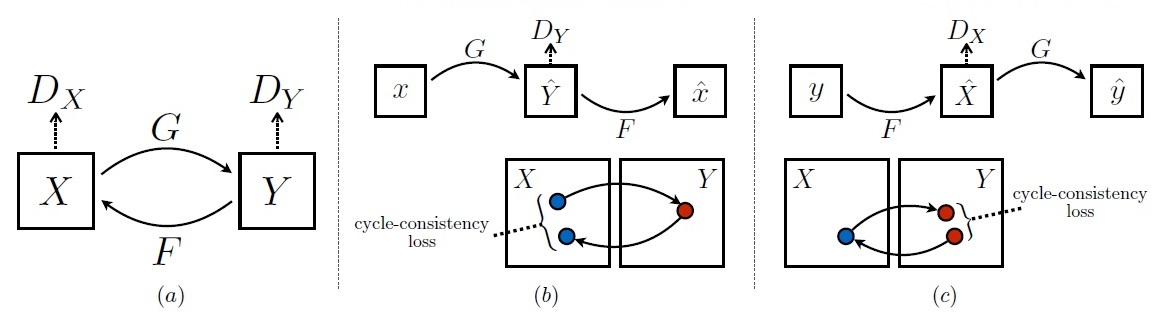
\includegraphics[width=5in,height=2in]{pic/fig3/fig3.jpg}
\caption{Two Mapping Functions with Cycle Consistency Loss in CycleGAN}
\end{center}
\label{fig:ccl_arch}
\end{figure}

The idea of \textit{Cycle Consistency} goes way back. It is an idea of determining the transitivity of two images where second image is the reconstruction of the first image. This transitivity is here denoted as \textit{Loss} in our case, where we use two \textit{Cycle Consistency Loss} as \textit{Forward \& Backward Cycle Consistency Loss}.\\
For our \textit{Cartoon-to-real} translation, if image, $c$ of domain $C$ is to be translated into domain $R$, through \textit{Generator} $G$, there must be another \textit{Generator} $F$ to translate the newly translated image $G(c)$ into $\hat{c}$ with a view to reconstructing $c$. From figure \ref{fig:ccl_arch}, if this \textit{Cycle Consistency Loss} is called \textit{Forward - Cycle Consistency Loss}, the opposite is called \textit{Backward - Cycle Consistency Loss}. It is defined using the following equations -
$$Forward\, Consistency\, Loss, L_{f\_cyc} = \frac{1}{m} \sum^m_{i=1}(F(G(c)) - c) $$
$$Backward\, Consistency\, Loss, L_{b\_cyc} = \frac{1}{m} \sum^m_{i=1}(G(F(r)) - r) $$
\\
A question may arise on why using \textit{Cycle Consistency Loss} solves the \textit{under-constraint} issue. 
\begin{figure}[!ht] 
 \begin{center}
\begin{tikzpicture}[
  node distance=0.8cm,
  >={Triangle[angle=60:1pt 2]},
  shorten >= 2pt,
  shorten <= 2pt,
  arrow/.style={
    ->,
    arrowblue,
    line width=2pt
  }
]
\ImageNode[label={90:Real Anime Pic}]{A}{pic/van/re2.png}
\node (B) [process,below of=A,node distance=3cm] {$D_r$};
\node (C) [process, below of=B,node distance = 2cm] {$\hat r$};
\node (D) [process, right of = C, xshift = 0.8cm] {F};
\node (E) [process, left of = C, xshift = -0.8cm] {G};
\node (F) [process, right of = D, xshift = 0.8cm] {$\hat c$};
\node (G) [process, left of = E, xshift = -0.8cm] {c};
\ImageNode[label={-90:Reconstructed},right=of F]{H}{pic/van/re4.png}
\ImageNode[label={-90:Real},left=of G]{I}{pic/van/re1.png}
\ImageNode[label={-90:Generated Anime Pic},below=of C]{I}{pic/van/re3.png}
\draw[arrow]
  (A) -- (B);
\draw[arrow]
  (C) -- (B); 
\draw[arrow]
  (G) -- (E); 
\draw[arrow]
  (E) -- (C);
\draw[arrow]
  (C) -- (D);
\draw[arrow]
  (D) -- (F);
\end{tikzpicture}
\caption{Architecture Of CycleGAN}
\end{center} 
\label{fig:example}
\end{figure}
The intuition is that for a general mapping of two images, \textit{Adversarial Loss} is great. However, it won't be able to specify the best image of the domain which should be mapped to the first image. On the other hand, \textit{Cycle Consistency Loss} can do this job. Let's think of a scenario, where someone wants to translate \textit{a garden image} to \textit{Monet Painting} using GAN. To his surprise, he finds out that when used only \textit{Adversarial Loss}, the machine translates the garden image with a random monet painting, kind of like figure \ref{fig:example} and on the other hand, when used \textit{Cycle Consitency Loss}, it shows the same contents of the garden which seems to be painted by \textit{Monet}. After some time, he finds out that, as \textit{Cycle Consistency Loss} minimizes the reconstruction loss of the image, the machine is bound to choose an image which is pretty similar to the garden image, as its loss must be the least. So, we can say that, \textit{Cycle Consistency Loss} binds the code to find out the best monet painting to be stylized.
\\

So, the total loss is - 
 $$L(G, F, D_c, D_r) = L_{adv} + L_{f\_cyc} + L_{b\_cyc}$$
 
\subsubsection{Network Architecture \& Training}
CycleGAN\cite{cyclegan} network consists of \textit{two}\textbf{ discriminator} networks and \textit{two} \textbf{generator} networks. The \textbf{discriminator} networks are used as \textbf{PathGANs}. Each \textbf{Generator} has \textit{three} sections: \textsc{Encoder, Transformer, Decoder} [Appendix \ref{appendix:En-Dec}]. Let's take a deeper look into the architecture.
\\
According to \textit{Zhao et al.}\cite{DBLP:journals/tci/ZhaoGFK17}, \textit{L1 Loss} performs best for \textit{Low frequency}[Appendix \ref{appendix:freq}] details, such as \textit{color-blotches, general tonal-distribution/contrast}. However, it fails at preserving \textit{High Frequency}[Appendix \ref{appendix:freq}] details, such as \textit{crisp, edge, texture} etc. Due to the use of \textit{L1 Loss} for \textit{Cycle consistency loss}, the model tends to lose its texture and crisp details. To avoid this situation, \textbf{discriminator} network is forced to model \textit{high frequency} structure. As a result, discriminator uses \textbf{PatchGAN} model which works as a fully collected layer checking a $N \times N$ patch of image every time whether that patch real or fake. In the case of CycleGAN, $70 \times 70$ pixel patch has been used. As texture and styles also work over patch, using \textbf{PatchGAN} preserve them. The architecture of \textbf{PatchGAN} is shown in Table \ref{Patch_Disc}.

\begin{table}[htbp]
\caption{PatchGAN Architecture}
\label{Patch_Disc}
\begin{tabular}{ll}
\hline
Layers &Discriminators \\
\hline
\hline
1 & CONV-(N64,K4,S2),  LeakyRelu \\
2 & CONV-(N128,K4,S2), InstanceNorm, LeakyRelu\\
3 & CONV-(N256,K4,S2), InstanceNorm, LeakyRelu\\
4 & CONV-(N512,K4,S2), InstanceNorm, LeakyRelu\\
\hline
\hline

\end{tabular}
\end{table}


We already know that each \textbf{Generator} consists of \textit{three} architectures within itself. When the input is fed into the network, it directly reaches the encoder, which extracts the representation model of the inputs. It has $three$ convolutional layers. After the final layer, it transforms the input into $256$ channels and passes it to the \textit{transformer} architecture. It is composed of a \textit{Residual Block}[Appendix \ref{appendix:resblock}] which has $6$ convolutional layers. The activated inputs are then expanded using \textbf{decoder} which uses $two$ \textit{deconvolutional layer}[Appendix. \ref{appendix:deconv}] to upsample the image and then a convolutional layer with 3 channels to output an \textbf{RGB} image. The architecture is shown in table \ref{gen_cyc}.
\begin{table}[htbp]
\caption{Generator Architecture of CycleGAN}
\label{gen_cyc}
\begin{tabular}{ll}
\hline
Layers &Generators\\
\hline
\hline
1 & CONV-(N64,K7,S1),InstanceNorm,Relu\\
2 & CONV-(N128,K3,S2),InstanceNorm,Relu\\
3 & CONV-(N256,K3,S2),InstanceNorm,Relu\\
4 & residual-(N256,K3)\\
5 & residual-(N256,K3)\\
6 & residual-(N256,K3)\\
7 & residual-(N256,K3)\\
8 & residual-(N256,K3)\\
9 & residual-(N256,K3)\\
10 & DCONV-(N128,K3,S1/2),fractional,strided, InstanceNorm, Relu\\
11 & DCONV-(N64,K3,S1/2),fractional,strided, IstanceNorm, Relu\\
12 & CONV-(N3,K7,S1),InstanceNorm,Relu\\
\hline
\hline
\end{tabular}
\end{table}

GAN has a tendency to show \textit{Mode Collapse}[Appendix \ref{mode_collapse}] which makes training so hard. To avoid \textit{Mode Collapse} in CycleGAN\cite{cyclegan}, last $50$ generated images are kept in a pool to train the discriminator instead of just training with the last generated image. This technique was acquired from \textit{Shrivastava et al.}\cite{DBLP:conf/cvpr/ShrivastavaPTSW17}.
\subsubsection{Limitations}

Although the output of generating cartoon images into real images look realistic, we can see from figure \ref{fig:lim} that, some of the outputs fail to preserve contents. From figure \ref{fig:lab_a}, CycleGAN\cite{cyclegan} outputs a firing sea whereas input image contains only sky. This has been the case for various outputs which is the biggest limitation of CycleGAN\cite{cyclegan} for our project.
\begin{figure}[!tbp]
\hspace{5cm}Input  \hspace{2.2cm} Output
\begin{center}
     \begin{subfigure}
    
         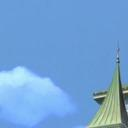
\includegraphics[scale = 0.7]{baaje_pic/Cycle/lat_real.png}
         \label{fig:lab_a}
     \end{subfigure}
     \begin{subfigure}
         
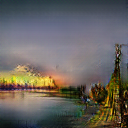
\includegraphics[scale = 0.7]{baaje_pic/Cycle/lat_fake.png}
     \end{subfigure}
\\

     \begin{subfigure}
    
        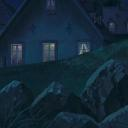
\includegraphics[scale = 0.7]{baaje_pic/Cycle/kds_real.png}
     \end{subfigure}
     \begin{subfigure}
         
        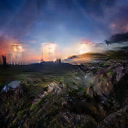
\includegraphics[scale = 0.7]{baaje_pic/Cycle/kdf_fake.png}
     \end{subfigure}
     \caption{Comparison}
\label{fig:lim}
\end{center}
\end{figure}

\subsection{UNIT}
Researchers of UNIT\cite{DBLP:journals/corr/LiuBK17} worked on an assumption known as shared latent space assumption, where a pair of corresponding images in different domains can be mapped to a same latent representation in a shared-latent space. The framework combined a variational autoencoder(VAE) and generative adversarial network (GAN). The adversarial training objective enforces the generator to transform corresponding images in two domains, while the variational autoencoders(VAE) make correlations between translated images with input images in the respective domain.\\ 

\subsubsection{Network Architecture \& Training}
The following abbreviation for ease of presentation is used: N=Neurons, K=Kernel size, S=Stride size. The transposed convolutional layer is denoted as DCONV. The residual basic block is denoted as RESBLK.

\begin{table}[htbp]
\caption{Network Architecture of Encoders and Generators MNIST $\rightarrow$ USPS}
\label{UNIT}
\begin{tabular}{ll}
\hline
Layers & Encoders\\
\hline
\hline
1 & CONV-(N64,K5,S2), BatchNorm, LeakyReLU \\
2 & CONV-(N128,K5,S2), BatchNorm, LeakyReLU \\
3 & CONV-(N256,K8,S1), BatchNorm, LeakyReLU \\
4 & CONV-(N512,K1,S1), BatchNorm, LeakyReLU \\
5 & CONV-(N1024,K1,S1)\\
\hline
Layers & Generators \\
\hline
\hline
1 & DCONV-(N512,K4,S2), BatchNorm, LeakyReLU \\
2 & DCONV-(N256,K4,S2), BatchNorm, LeakyReLU \\
3 & DCONV-(N128,K4,S2), BatchNorm, LeakyReLU \\
4 & DCONV-(N64,K4,S2), BatchNorm, LeakyReLU \\
5 & DCONV-(N3,K1,S1), TanH \\
\hline
\hline

\end{tabular}
\end{table}

\begin{table}[htbp]
\caption{Network Architecture of Discriminators MNIST $\rightarrow$ USPS}
\label{UNIT1}
\begin{tabular}{ll}
\hline
Layers & Discriminators\\
\hline
\hline
1 & CONV-(N20,K5,S1), MaxPooling-(K2,S2) \\
2 & CONV-(N50,K5,S1), MaxPooling-(K2,S2) \\
3 & FC-(N500), ReLU, Dropout \\
4a & FC-(N1), Sigmoid \\
4b & FC-(N10), Softmax \\

\hline
\hline

\end{tabular}
\caption{Network Architecture of Discriminators SVHN $\rightarrow$ MNIST}
\label{UNIT1}
\begin{tabular}{ll}
\hline
Layers & Discriminators\\
\hline
\hline
1 & CONV-(N64,K5,S1), MaxPooling-(K2,S2) \\
2 & CONV-(N128,K5,S1), MaxPooling-(K2,S2) \\
3 & CONV-(N256,K5,S1), MaxPooling-(K2,S2) \\
4 & CONV-(N512,K5,S1), MaxPooling-(K2,S2) \\
5a & FC-(N1), Sigmoid \\
5b & FC-(N10), Softmax \\

\hline
\hline

\end{tabular}

\end{table}

\subsubsection{Limitations}
In UNIT\cite{DBLP:journals/corr/LiuBK17} outputs, the images tend to be soft on the surfaces of the outputs. In real world images, the surfaces are not that smooth as it is in UNIT outputs. Real world images tends to be less sharpen on the edges and more crisp on the surface.  

\begin{figure}
\hspace{5cm}Input  \hspace{2.2cm} Output
\begin{center}
     \begin{subfigure}
    
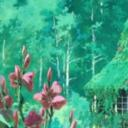
\includegraphics[scale = 0.7]{baaje_pic/UNIT/286_c.jpg}
         \label{fig:ulab_a}
     \end{subfigure}
     \begin{subfigure}
         
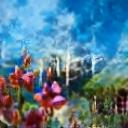
\includegraphics[scale = 0.7]{baaje_pic/UNIT/286_r.jpg}
     \end{subfigure}
\\

     \begin{subfigure}
    
        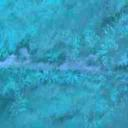
\includegraphics[scale = 0.7]{baaje_pic/UNIT/143_c.jpg}
     \end{subfigure}
     \begin{subfigure}
         
        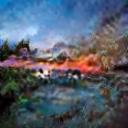
\includegraphics[scale = 0.7]{baaje_pic/UNIT/143_r.jpg}
     \end{subfigure}
     \caption{Comparison}
\label{fig:lim_un}
\end{center}
\end{figure}
\subsection{SingleGAN}
We have already known about two models which consist of multiple generators and discriminators. However, using multiple generators might be ineffective and inefficient. To reduce inefficiency, researchers of SingleGAN \cite{SingleGAN} worked on producing unpaired image translation using a \textbf{Single Generator}. Basically, it is a multi-domain image-to-image translation using \textit{Single Generator} and multiple \textit{Generative Adversarial}  Learning Objects. \\

Intuitively, while translating an image of one domain to another, there exists some common features, such as content, edge of the first domain which will retain its position even after translation. From figure \ref{fig: common}, we get an idea how this works where $3$ of domain 1 and domain 2 share common features which at this point is clearly the edge.
\begin{figure}[!htp] 
\centering
    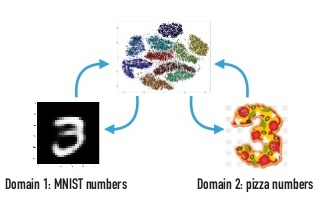
\includegraphics[scale = 1.3]{shared_domain_singleGAN.jpg}
    \caption{In this figure, $3$ of domain $1$(\textit{MNIST Dataset) and pizza-looking $3$ of domain $2$ share common features.}}
\label{fig: common}
\end{figure}
\\
Researchers of singleGAN use this intuition for their work. They generalize the model by sharing these features. For specific domain mapping, an domain distribution, retrieved by auxiliary information, is used . \\
For cartoon to real translation, if the auxiliary information is $Z$, $C$ is cartoon domain and $R$ is real domain, we can define the functions as - 
$$x_C^{fake} = G(x_R, Z_c)$$
$$x_R^{fake} = G(x_C, Z_R)$$

Here, domain code is retrieved using \textit{Central Biasing
Instance Normalization (CBIN)}\cite{chen2016infogan} with the help of auxiliary information.

\subsubsection{Loss Functions}
\textbf{SingleGAN} uses $two$ loss functions. These are \textit{Adversarial Loss} and \textit{Cycle Consistency Loss}.\\
As it gets to use a single generator to translate one image to another, it uses $one$ \textit{Adversarial Loss} for each domain translation. In our case, where we have $two$ domains $C$ and $R$, the loss will be as followiing -
$$L_{adv}(G, D_C) = \E_{x_C}[log(D_C(x_C))] + \E_{x_R, Z_C}[log(1 - D_C(G(x_R, Z_C))]$$
$$L_{adv}(G, D_R) = \E_{x_R}[log(D_R(x_R))] + \E_{x_C, Z_R}[log(1 - D_R(G(x_C, Z_R))]$$
As mentioned in \ref{cyc_adv} and \ref{cyc_ccl}, the same problem may also happen in SingleGAN condition. Due to being \textit{unconstraint}, an additional loss, Cycle Consistency loss is used. For our case, the loss will be -
$$L_{cyc_{sing}} = \E_{x_C}[||x_C - G(G(x_C, Z_R), Z_C)||_1] + \E_{x_R}[||x_R - G(G(x_R, Z_C), Z_R)||_1]$$
So, the final loss is -
$$L = L_{adv}(G, D_C) + L_{adv}(G, D_R) + L_{cyc_{sing}}$$

\subsubsection{Network Architecture \& Training}
Generator G uses the ResNet\cite{DBLP:journals/corr/HeZRS15} structure with an encoder-decoder framework, which contains two stride-2 convolution layers for downsampling, six residual blocks and two stride-2 transposed convolution layers for upsampling. All the normalization layers are replaced except upsampling layers. For the discriminators D, two discriminators\cite{DBLP:journals/corr/IsolaZZE16} are used to discriminate the real and fake images in different scales.

\subsubsection{Limitations}
Unfortunately, of all models, \textbf{SingleGAN} performed the worst. The color scheme of the output is totally faded. We can see examples from \ref{fig:lim_sing}
\begin{figure}[!hb]
\hspace{5cm}Input  \hspace{2.2cm} Output
\begin{center}
     \begin{subfigure}
    
         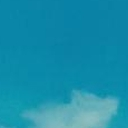
\includegraphics[scale = 0.7]{baaje_pic/SingleGAN/image076_D0.jpg}
         \label{fig:labs_a}
     \end{subfigure}
     \begin{subfigure}
         
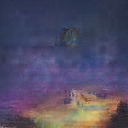
\includegraphics[scale = 0.7]{baaje_pic/SingleGAN/image076_0to1.jpg}
     \end{subfigure}
\\

     \begin{subfigure}
    
        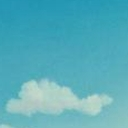
\includegraphics[scale = 0.7]{baaje_pic/SingleGAN/image259_D0.jpg}
     \end{subfigure}
     \begin{subfigure}
         
        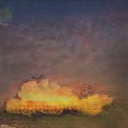
\includegraphics[scale = 0.7]{baaje_pic/SingleGAN/image259_0to1.jpg}
     \end{subfigure}
     \caption{Comparison}
\label{fig:lim_sing}
\end{center}
\end{figure}

